\subsection{Notation}
The basic building block of a QC is the \textit{qbit}. Resembling the binary representation in CC, the qbit is defined as a two-level system. In the canonical/standard/Pauli basis, we express the basis states as
\begin{align*}
    \ket{0} = \begin{pmatrix}
        1 \\
        0
    \end{pmatrix}, \ket{1} = \begin{pmatrix}
        0 \\ 
        1
    \end{pmatrix}.
\end{align*}
Despite the similarity to bits, a qbit is allowed to be in a superposition of the two basis states, meaning that 
\begin{align*}
    \ket{\psi} = c_0 \ket{0} + c_1 \ket{1}, \hspace{20px} c_0,c_1 \in \mathbb{C}
\end{align*}
is also a valid qbit, constrained to normalization $|c_0|^2 + |c_1|^2 = 1$. The modulus of the coefficients $c_0,c_1$ are through the Born rule interred as the point probability of measuring basis state $\ket{0}$ and $\ket{1}$ respectively, mirroring probability vectors. However, the qbits $\set{\ket{\psi}_i}$ are expressed through the coefficients $\set{c_i}$ and not their modulus, allowing both negative and complex values, resulting in the possibility for both constructive and destructive interference when added together.

We are however not only limited to a single qbit. Composite systems of two-level qbits can be created, mathematically expressed as tensor products between states. Considering the Pauli basis $\set{\ket{0},\ket{1}}$, we can create a new basis $\set{\ket{00},\ket{01},\ket{10},\ket{11}}$ through the operation
\begin{align}
    \ket{ij} = \ket{i} \otimes \ket{j} \hspace{20px} i,j=0,1. \label[eq]{eq:theo:pauli_matricies_definition}
\end{align}
The above procedure can be repeated for more than two qbits. In the realm of QC, the most important operators are the Pauli matrices, often referred to the $X,Y$ and $Z$ \textit{gates} 
\begin{align}
    X = \begin{pmatrix}
        0 & 1 \\
        1 & 0
    \end{pmatrix}, Y = \begin{pmatrix}
        0 & -i \\
        i & 0
    \end{pmatrix}, Z = \begin{pmatrix}
        1 & 0 \\
        0 & -1
    \end{pmatrix}
\end{align}
Just as with qbits, we can through the tensor product compose operators acting on multiple qbits. To avoid potential confusion between multiple operators being applied and composite operators, a subscript on these operators will be added. For instance, a three qbit operator can be constructed as
\begin{align}
    X_1 Z_3 = X \otimes I \otimes Z 
\end{align} 
Where $I$ is the $2 \times 2$ identity matrix. Here $X_1 Z_3$ applied to a three qbit state applies $X$ to the first qbit, does nothing with the second and applies $Z$ on the third.
% \begin{align*}
%     \ket{+} = \frac{1}{\sqrt{2}} (\ket{0} + \ket{1}) \\ 
%     \ket{-} = \frac{1}{\sqrt{2}} (\ket{0} - \ket{1})
% \end{align*}

\subsection{Basics of Quantum Computing}
In the introduction, vague outlines of the functionality of QC is presented. In this section, the circuits and representation will be presented with a elementary example of circuits and states. A Greenberger-Horne-Zeilinger(GHZ) State is a  fully entangled set of three or more quantum bits, or qbits. For two qbits, this is called a Bell-state. It can be encoded by applying a Haddamard gate to the primary gate, and CNOT gates to the subsequent. In matrix representation these operations are
\begin{equation}
    H = \begin{pmatrix}
    1 & 1 \\
    1 & -1 
    \end{pmatrix} \qquad 
    CNOT = \begin{pmatrix}
    1 & 0 & 0 & 0 \\
    0 & 1 & 0 & 0 \\
    0 & 0 & 0 & 1 \\
    0 & 0 & 1 & 0 
    \end{pmatrix}
\end{equation}
\begin{figure}
    \centering
    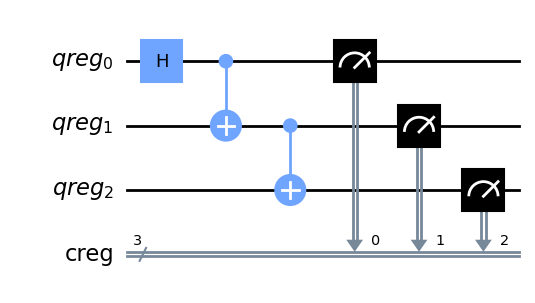
\includegraphics[width=\linewidth]{figs/GHZ.png}
    \caption{The circuit needed to initialize the GHZ state for three qubits.}
    \label{fig:GHZ_circ}
\end{figure}
Hadamard gates changes the basis of the gate between Pauli Z and Pauli X basis. CNOT changes the affected gate, based on the state of the control state. Visually, in a circuit, this can be presented as shown in Fig(\ref{fig:GHZ_circ}).
The result is a full entanglement, as seen in Fig(\ref{fig:qshpere}), where the outcome of any measurement on any qbit, will ascertain the outcome of all other measurements, as shown in Fig(\ref{fig:GHZ_measure}).
\begin{figure}
    \centering
    \begin{subfigure}{0.48\textwidth}
        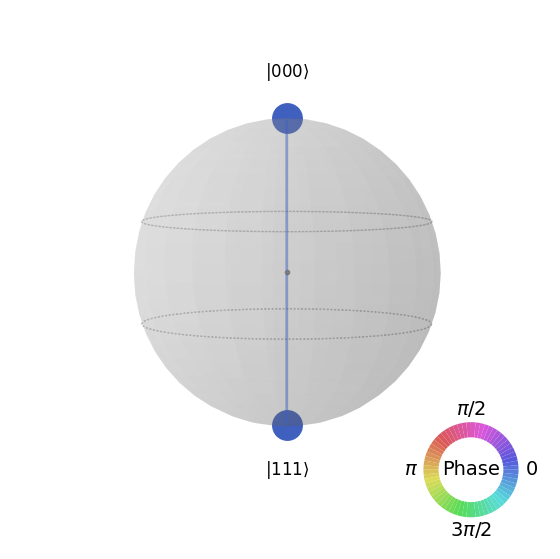
\includegraphics[width=\textwidth]{figs/GHZ qsphere.png}
        \caption{The Bloch-sphere representation of the GHZ state, given three qubits. It is strictly entangled, by their parallell nature.}
        \label{fig:qshpere}
    \end{subfigure}
    \hfill
    \begin{subfigure}{0.48\textwidth}
        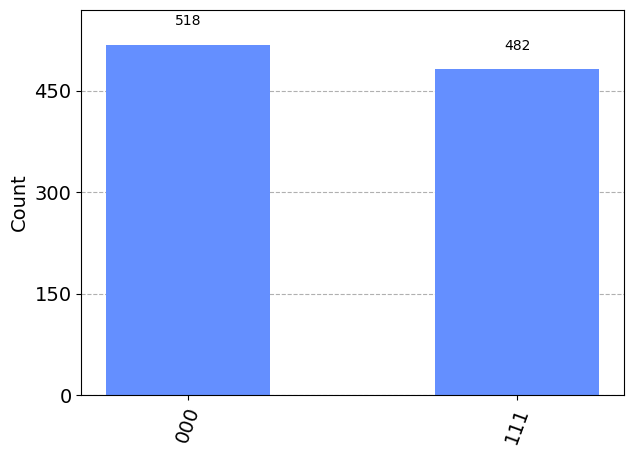
\includegraphics[width=\textwidth]{figs/GHZ Counts.png}
        \caption{The outcome of measurements of the GHZ state with three qubits.}
        \label{fig:GHZ_measure}
    \end{subfigure}
\end{figure}
\subsection{Variational Principle}
The Rayleig-Ritz Variational Method claims that for a given Hamiltonian operator, \textbf{H}, the expectation value of a given state has a lower bound on the energy $E_0$, such that
\begin{equation}
    \frac{\bra{a}\boldsymbol{H}\ket{a}}{\braket{a}} \geq E_0
\end{equation}
This is a crucial method in perturbation theory, as it allows for the ability to approximate the lower bounds of the lowest eigenvalue of the Hamiltonian. It is the essential principle of the Variational Quantum Eigensolver. 

\subsection{Variational Quantum Eigensolver}
The Variational Quantum Eigensolver(VQE) takes on applying the Variational Principle, described above, minimizing the energy of 
\begin{equation}\label{VQE}
    E_{temp} = \frac{\bra{a}\boldsymbol{H}\ket{a}}{\braket{a}}
\end{equation}
with regards to altering the state $\ket{a}$. This is achieved by applying an ansatz to the initial state, in order to get an output eigenvalue, which further can be minimized. The ansatz takes \textit{n} Quantum Bits (qbits) and \textit{n} free parameters, $\theta_i$. The goal of the algorithm is to alter the parameters $\theta_i$ in order to achieve the optimal the minimal energy of the system, as computed in Eq. (\ref{VQE}). A schematic of the process is shown in Fig(\ref{fig:VQE_scheme}). The ansatz conjectured by Hlatshwayo et al. \cite{} is shown in Fig. (\ref{fig:ansatz}). \begin{figure}
    \centering
    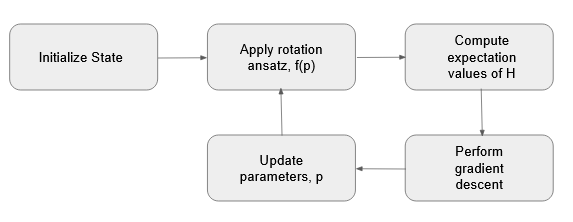
\includegraphics[width=\linewidth]{figs/VQE.PNG}
    \caption{A schematic of the process of Variational Quantum Eigensolvers.}
    \label{fig:VQE_scheme}
\end{figure}
\begin{figure}
    \centering
    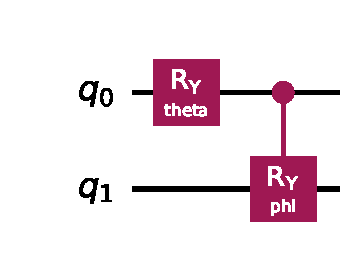
\includegraphics[width=\linewidth]{figs/ansatz.pdf}
    \caption{The ansatz for the VQE scheme applied for N = 4. }
    \label{fig:ansatz}
\end{figure}

\subsection{Pauli Encoding Hamiltonians}
To apply a specific system to VQE, the Hamiltonian must be re-written in terms of a sum of \textit{Pauli strings}. Considering the identity $I$ and the three Pauli matrices $X, Y, Z$, we construct a specific term as a tensor product of these $P_i$. For an $n$-qubit system, we require $n-1$ tensor products. Combined with a weight $w_i$, the Hamiltonian must be written in the from
\begin{align}
    H = \sum_i w_i P_i \label[eq]{eq:theo:pauli_encoding_general}
\end{align}
For a general two-body Hamiltonian, this task can serve challenging. Many schemes exists for this purpose, such as the Jordan-Wigner transformation \citep{steudtnerMethodsSimulateFermions2019}. For the Lipkin model, an easier approach is available since the Hamiltonian can be written as products of the number and spin operators.
